\begin{figure}
	\centering
	\begin{subfigure}{0.45\linewidth}
		\centering
		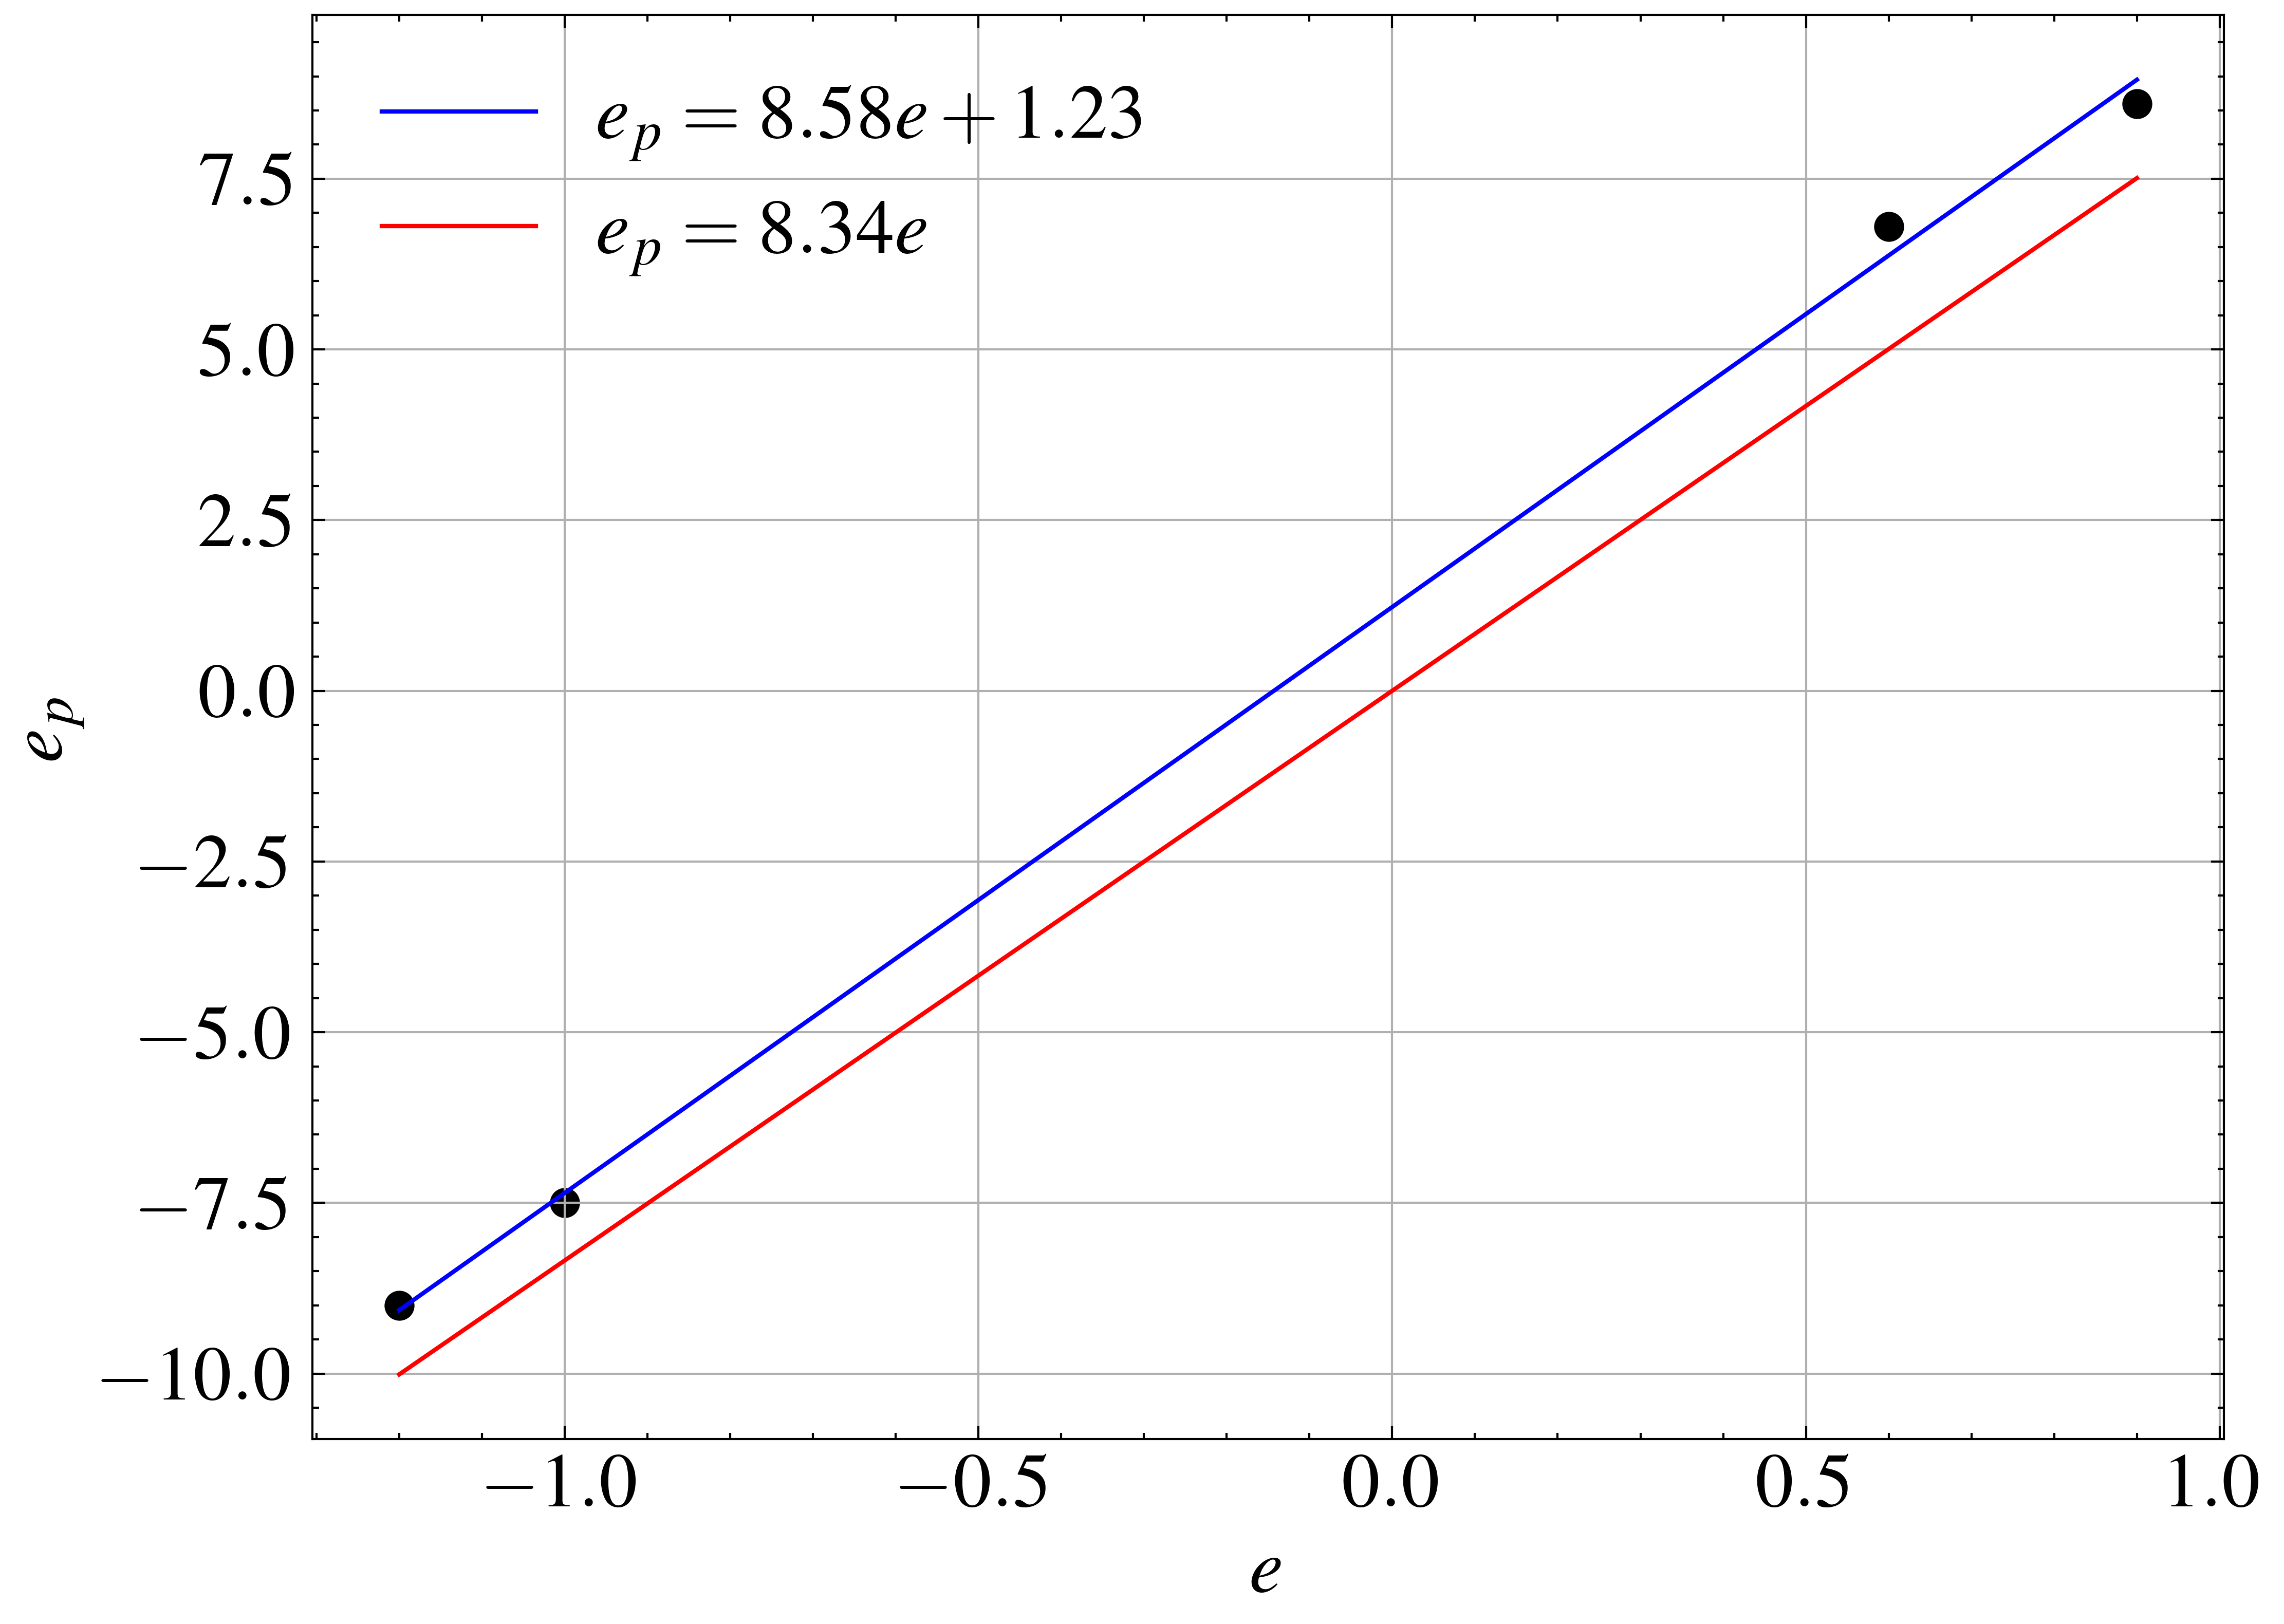
\includegraphics[width=\linewidth]{src/figures/e-e_p-relation/e-e_p-relation-60.png}
		\subcaption{$P=60$}\label{fig:e-e_p-relation-60}
	\end{subfigure}
	\begin{subfigure}{0.45\linewidth}
		\centering
		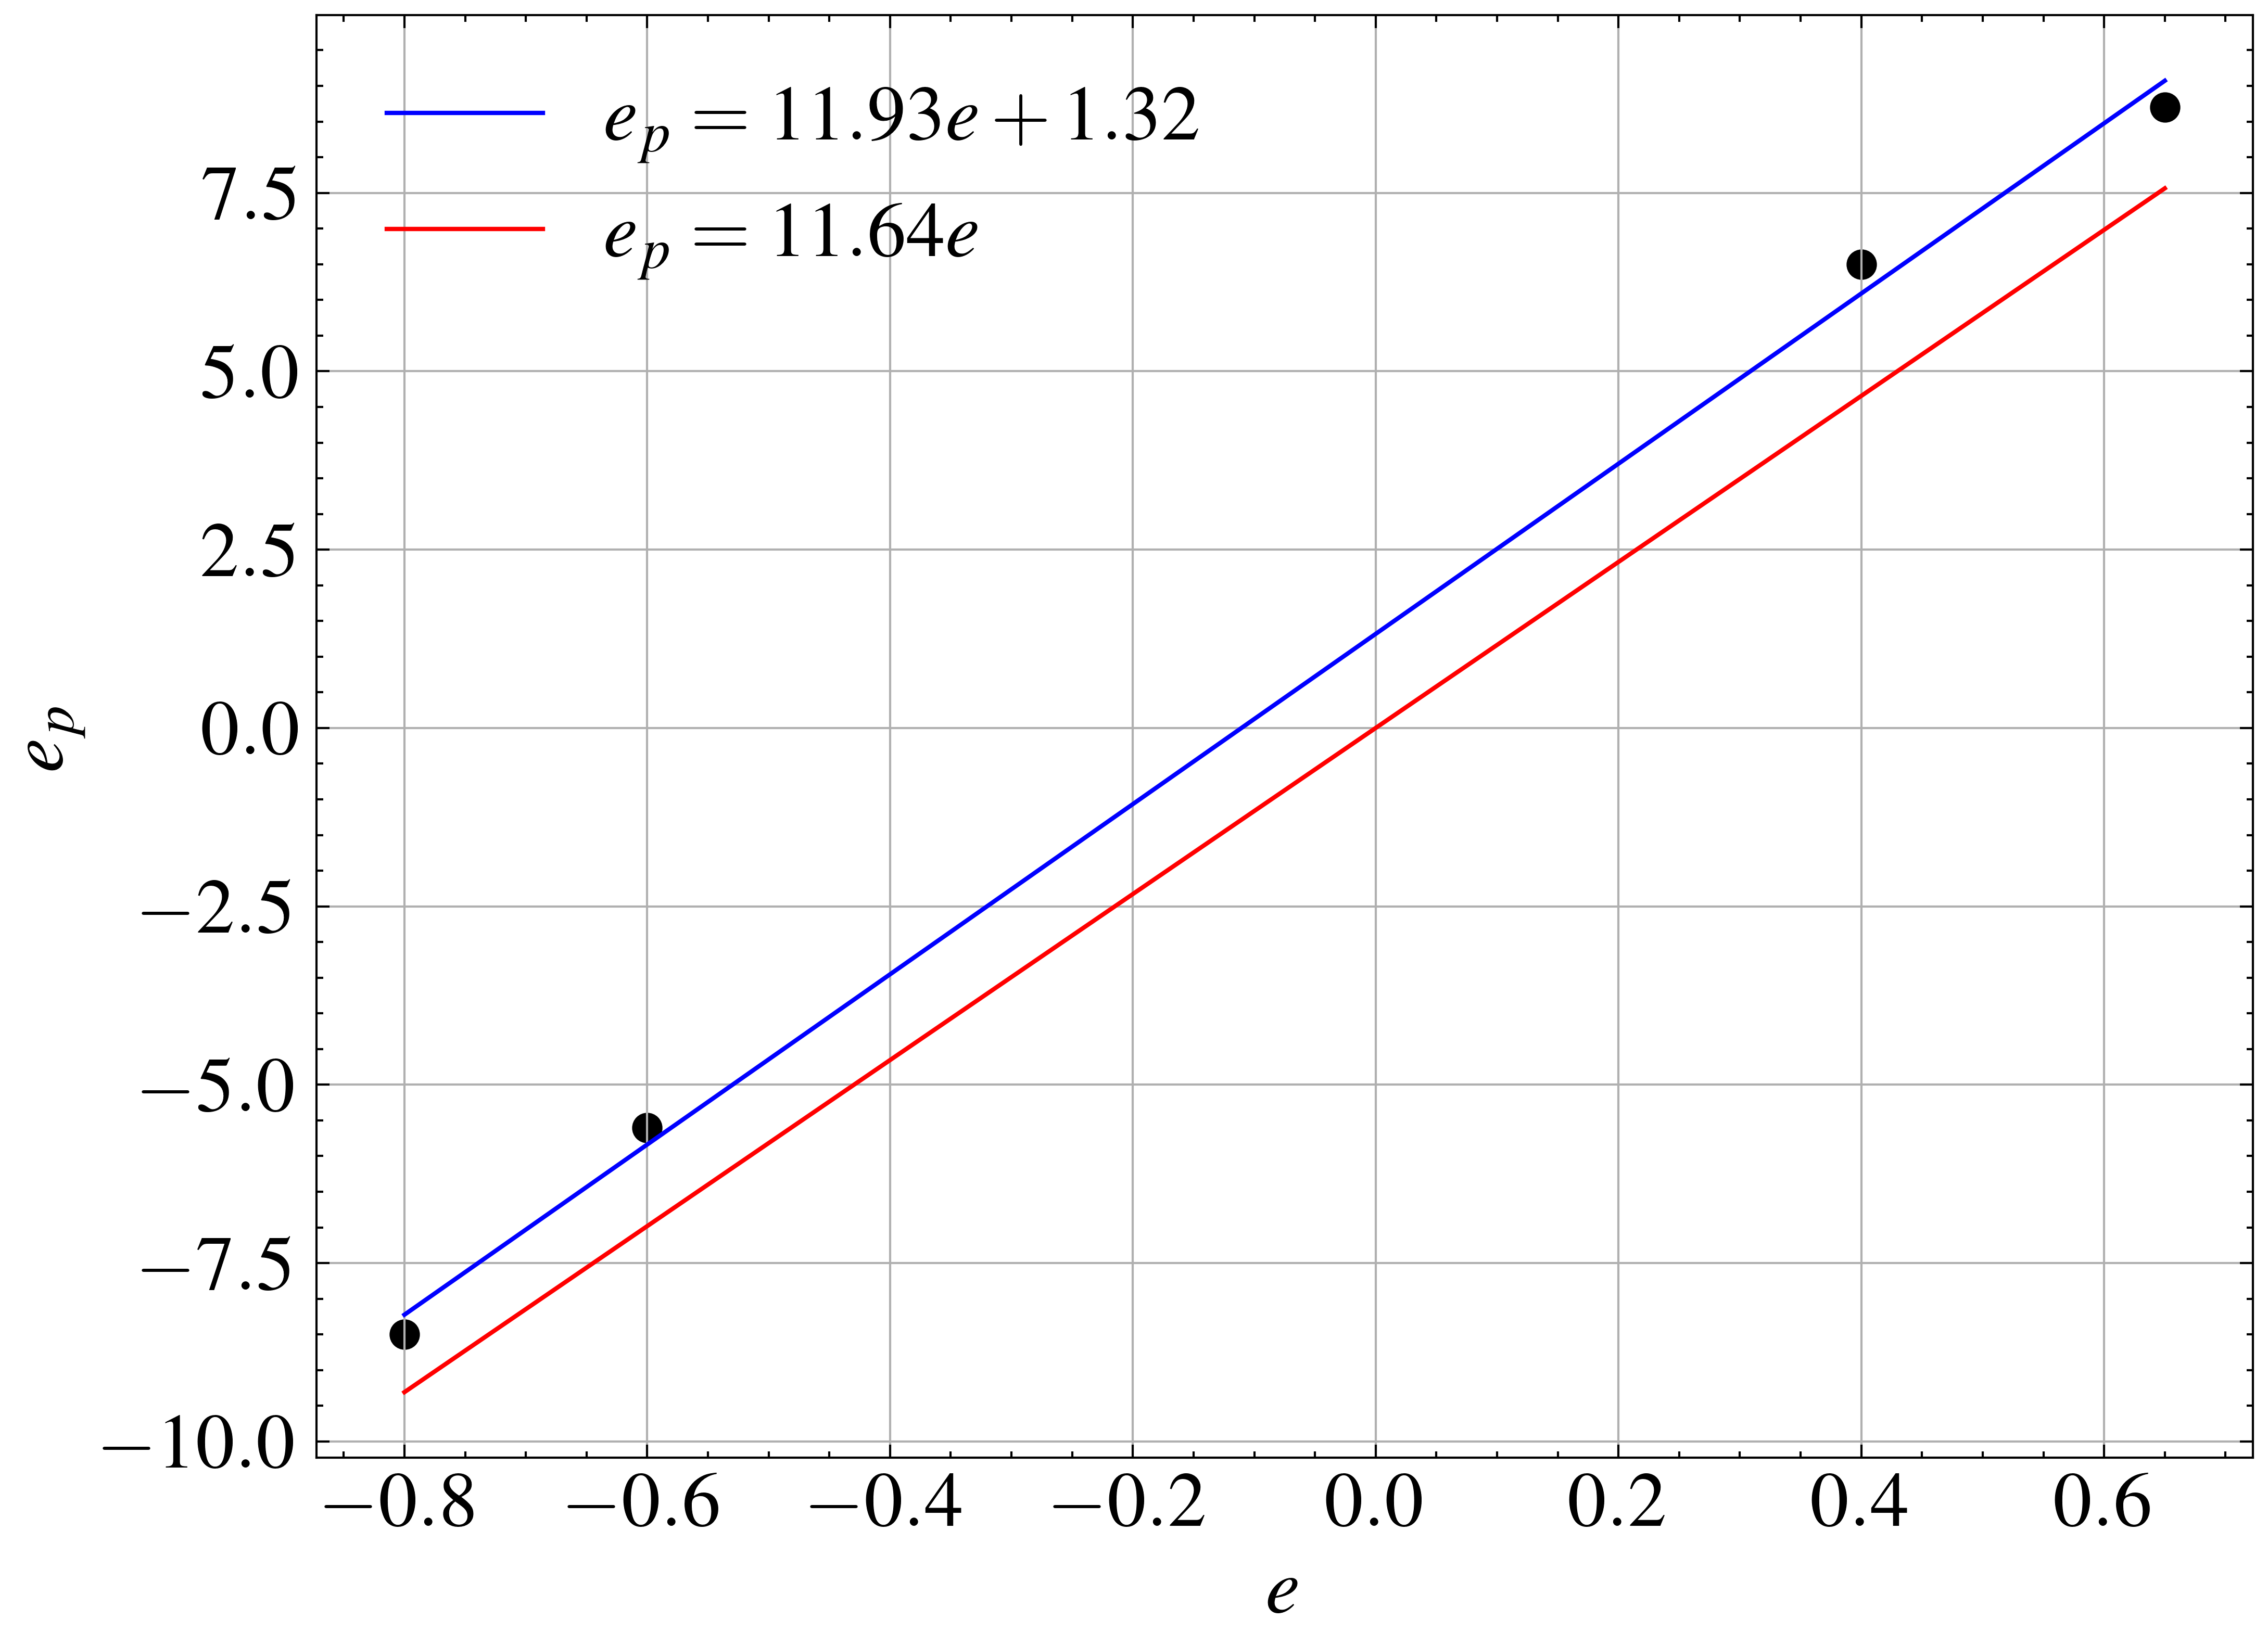
\includegraphics[width=\linewidth]{src/figures/e-e_p-relation/e-e_p-relation-80.png}
		\subcaption{$P=80$}\label{fig:e-e_p-relation-80}
	\end{subfigure}
	\begin{subfigure}{0.45\linewidth}
		\centering
		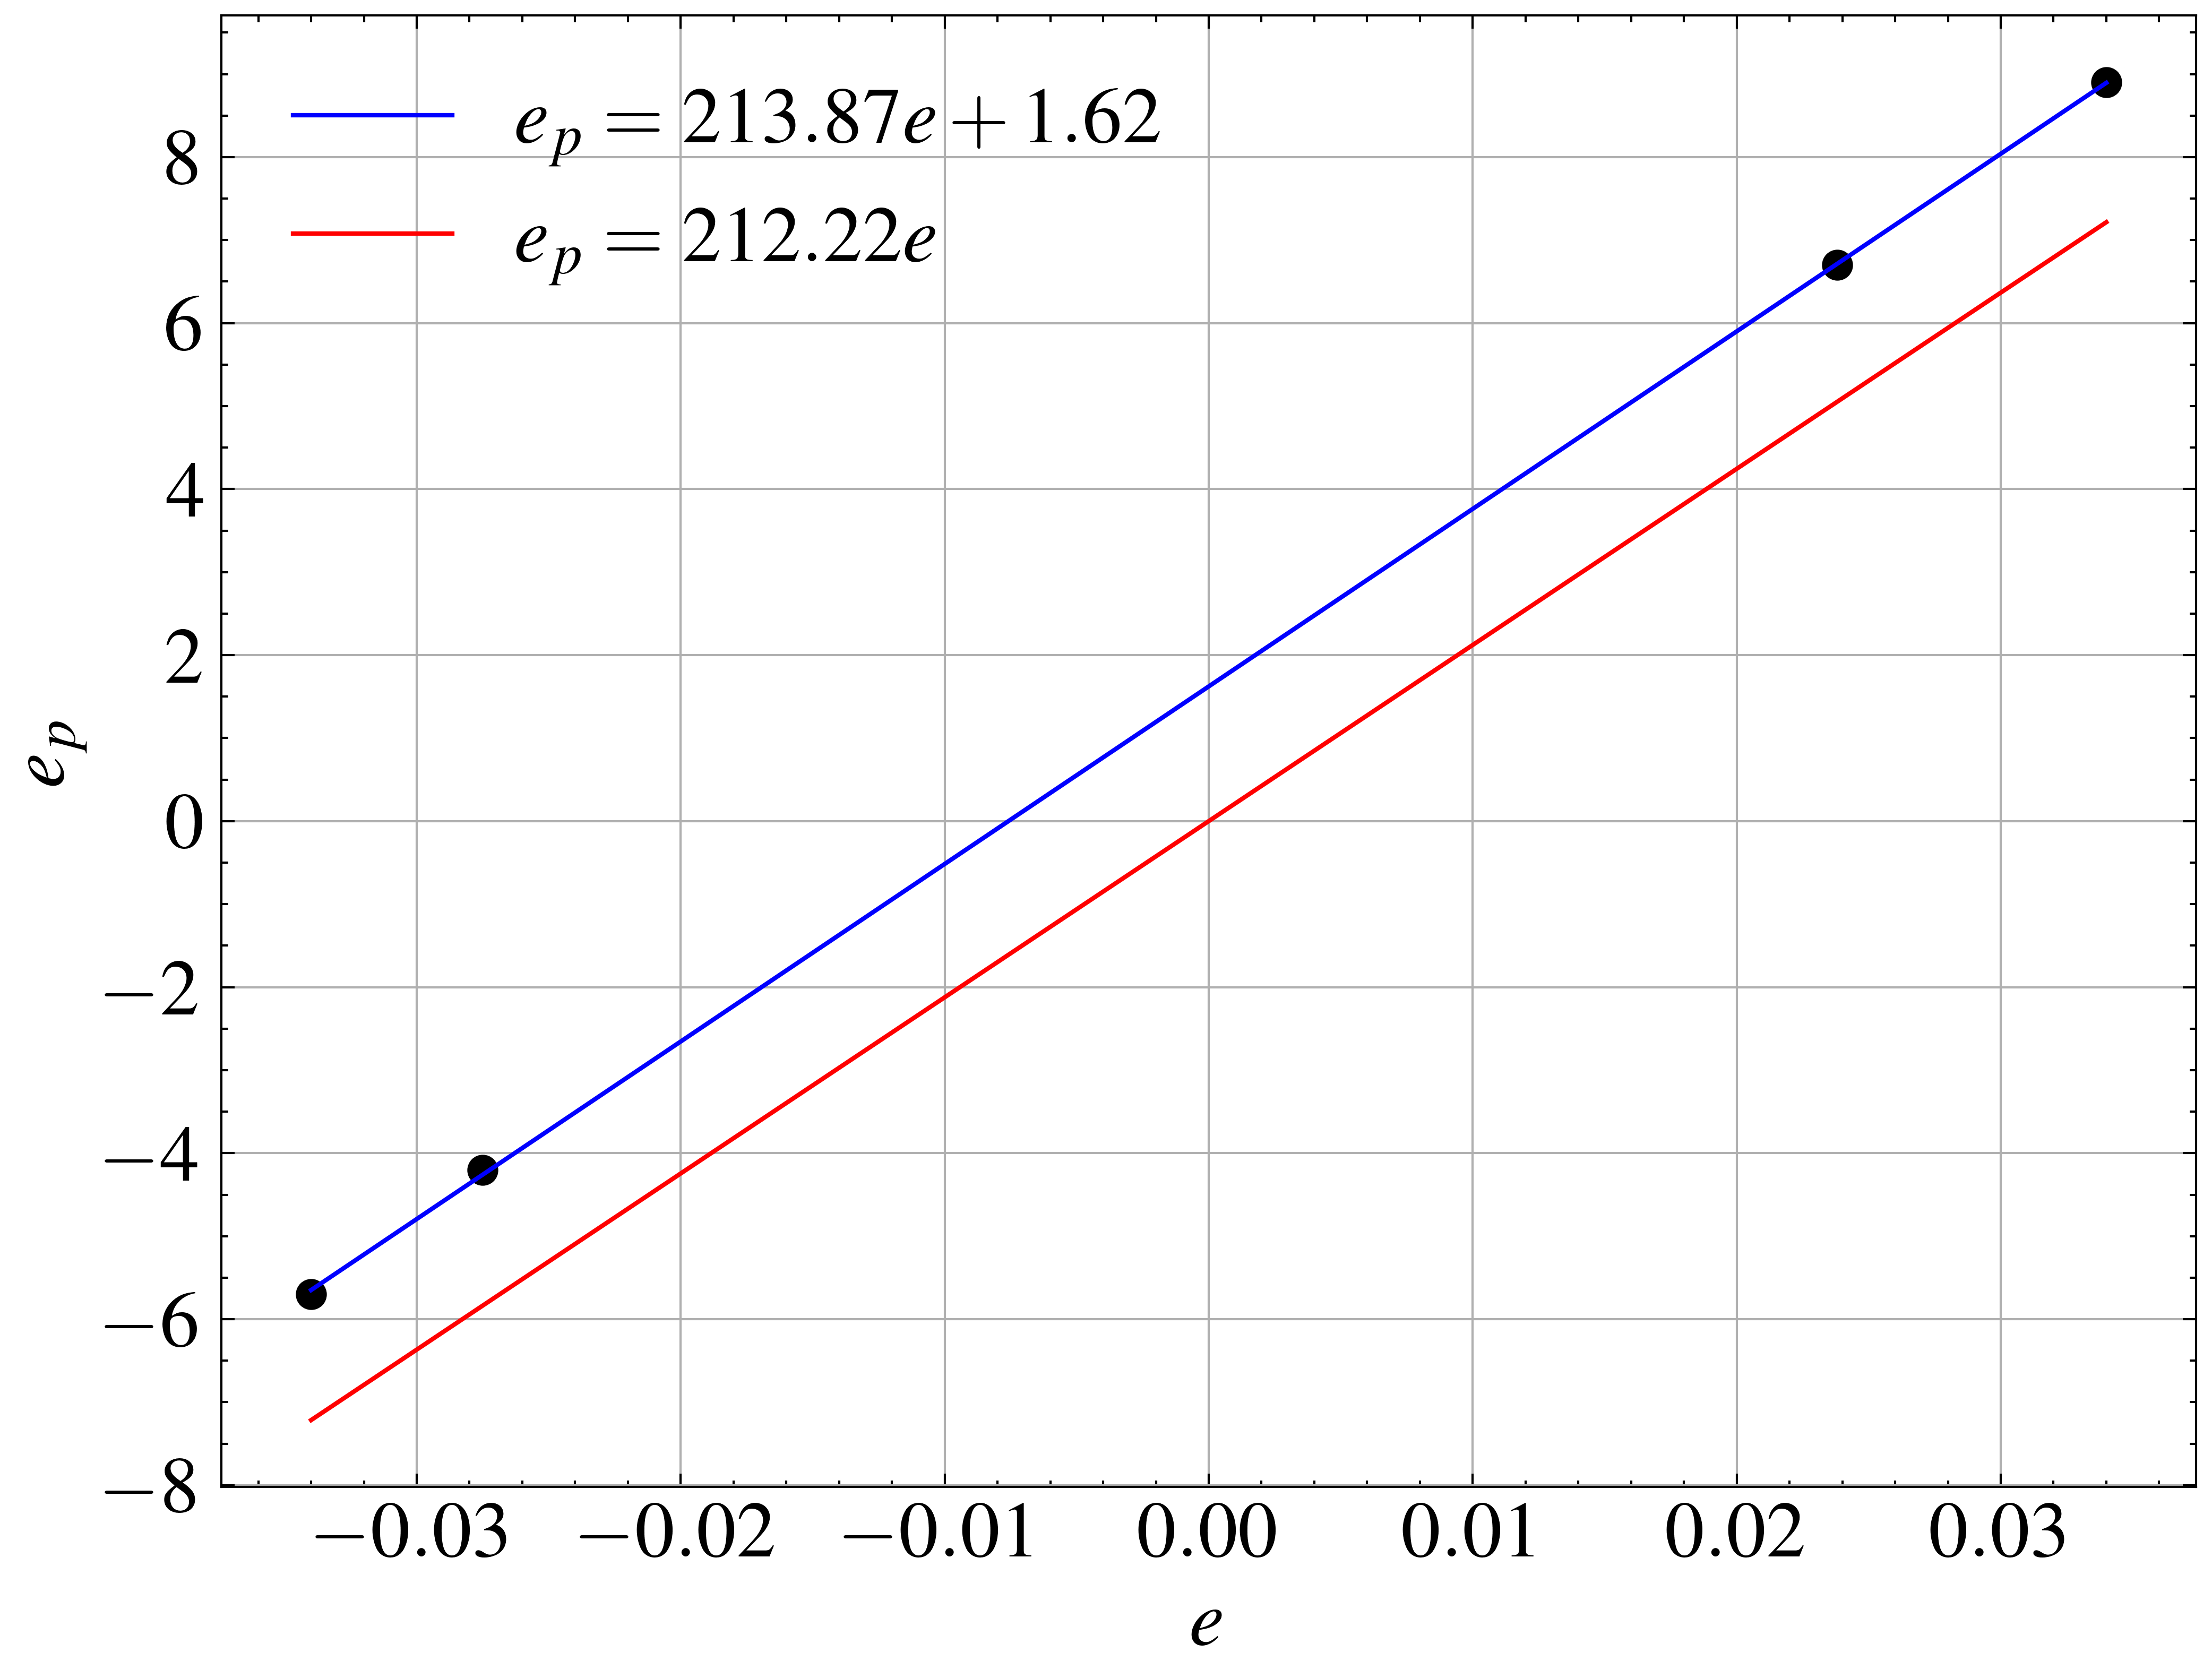
\includegraphics[width=\linewidth]{src/figures/e-e_p-relation/e-e_p-relation-100.png}
		\subcaption{$P=100$}\label{fig:e-e_p-relation-100}
	\end{subfigure}

	\caption{$e$と$e_p$の関係}\label{fig:e-e_p-relation}
\end{figure}
